\documentclass[./\jobname.tex]{subfiles}
\begin{document}
\chapter {Experiment 3: Gauss-Sinus Kernel}
\label{chap:experimet_3}

Up until now, the results on \gls{pde} 5 were always considerably worse than on all other testbed functions. The idea discussed in this chapter is the usage of a new kernel. The Gauss-Sinus Kernel, also abbreviated with \gls{gsk}, was introduced in chapter \ref{chap:gsin_kernel}. Theoretically, the kernel should be able to solve the testbed \gls{pde}s 0A and 0B exactly.  

\section{Hypotheses}
As stated in chapter \ref{chap:ex0_pde5} attempting to solve \gls{pde} 5 with more \gls{nfe} results in a worse solution quality. The adaptive kernel scheme could not improve the results. This means that the fitness function must be reconsidered. A simple approach to change the fitness function is by introducing a new kernel type. The \gls{gsk} has the features of a Gauss kernel and a sine function and is potentially able to approximate more \gls{pde} solutions. The idea of the sine function is to help with the circular features of the wave front. 

This experiment tries to answer the question if the new \gls{gsk} kernel type can effectively improve the results on \gls{pde} 5. Further, it should at least maintain the solution quality on all other testbed \gls{pde}s. 

\section{Experiment Setup}

As stated in the experiments chapters before, machine 1 performs the time and memory experiments at $10^4$ \gls{nfe}. Similar, machine 2 runs the experiment at the full computational budget of $10^6$ \gls{nfe}. The Wilcoxon test from appendix \ref{chap:apendix_post_proc} is used to show statistical significance. Because the last experiment was not entirely conclusive, only a memetic pJADE without kernel-adaption is tested. Since the new kernel has 6 parameters, the dimension and the population size changes. To ensure that the algorithm is able to solve \gls{pde} 0A, 5 \gls{gsk} are used. This results in a dimension of 30 parameters and a population size of 60. All other experimental parameters are taken from the table \ref{tab:ci_parameter}. 

\section{Result}

The box plots in figure \ref{fig:pJADEgsk_time_boxplot} compares the relative execution time of the memetic pJADE with the \gls{fem} solver. The results seen in this graph are obtained after $10^4$ \gls{nfe} on machine 1. Similar, the data in figure \ref{fig:pJADEgsk_memory_boxplot} compares the memory consumption of both algorithms. 

The memory consumption boxplot exhibits many outliers, where some even indicate a memory usage of 0 Mbyte. This is not expected and might result from technical difficulties. Thus, when comparing the results, only the median should be considered. 

The following table show the statistical test. The comparison between the \gls{gsk} and the \gls{gak} on the memetic parallel JADE is shown in table \ref{tab:compare_mpj_mpjgsk_10^6}. The comparison is done with a budget of $10^6$ \gls{nfe}. 

\begin{figure}[H]
	\centering
	\noindent\adjustbox{max width=0.66\linewidth}{
		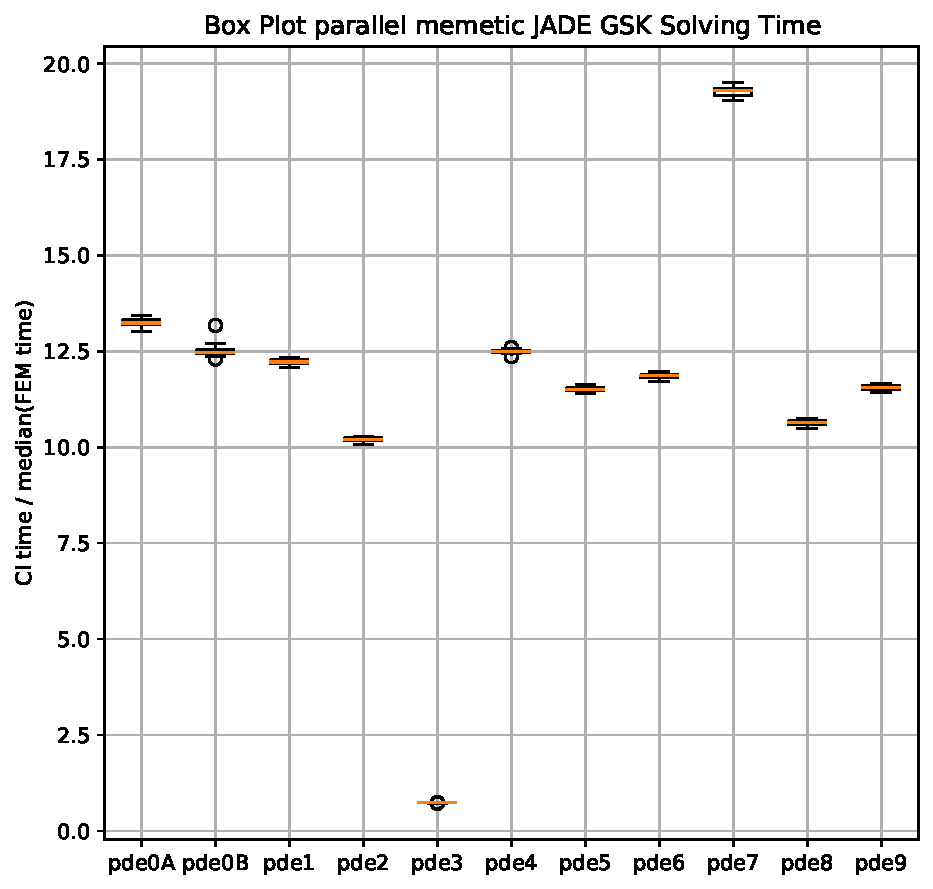
\includegraphics[width=\textwidth]{../../code/experiments/experiment_3/time_boxplot_ci_exp3.pdf}
	}
	\unterschrift{Relative solving time results of parallel memetic JADE with \gls{gsk} after $10^4$ \gls{nfe}.}{}{}
	\label{fig:pJADEgsk_time_boxplot}
\end{figure}



\begin{figure}[H]
	\centering
	\noindent\adjustbox{max width=0.66\linewidth}{
		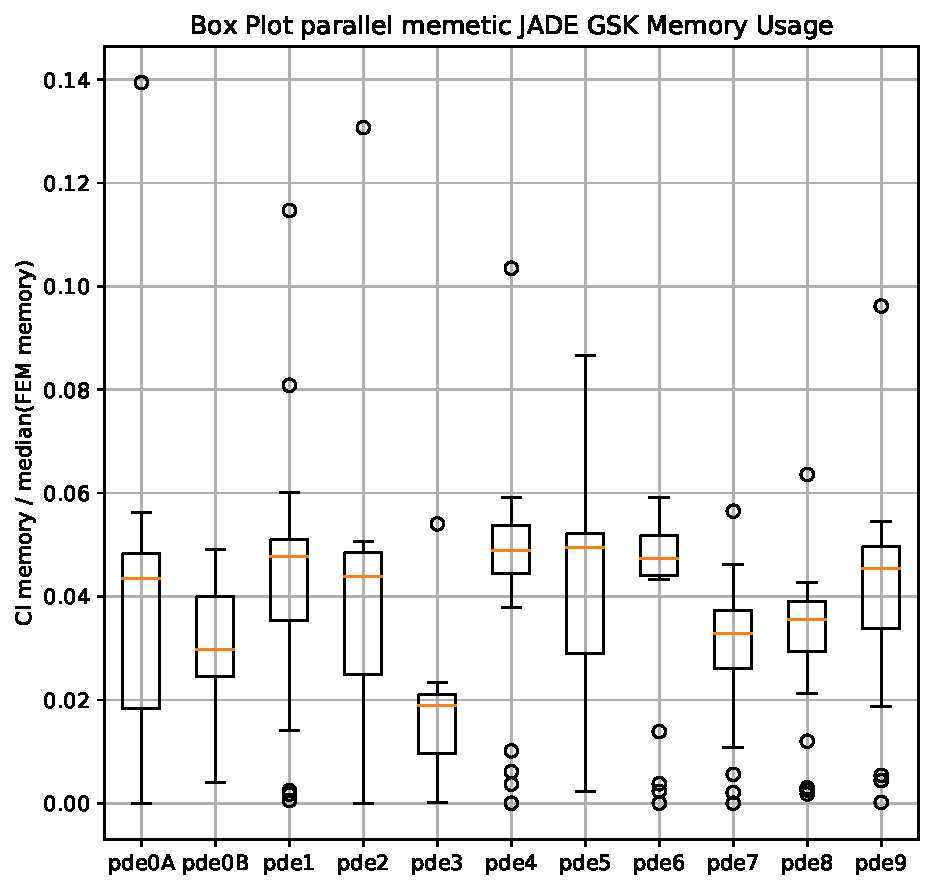
\includegraphics[width=\textwidth]{../../code/experiments/experiment_3/mem_boxplot_ci_exp3.pdf}
	}
	\unterschrift{Relative memory usage results of parallel memetic JADE with \gls{gsk} after $10^4$ \gls{nfe}.}{}{}
	\label{fig:pJADEgsk_memory_boxplot}
\end{figure}


\begin{table}[H]
	\centering
	\noindent\adjustbox{max width=\linewidth}{
		\begin{tabular}{|c|c|c|c|c|l|}
			
			\hline
			\rowcolor[HTML]{\farbeTabA}
			
			Algorithm & \multicolumn{2}{|c|}{parallel JADE \gls{gak} $10^6$ \gls{nfe}} & \multicolumn{2}{|c|}{parallel JADE \gls{gsk} $10^6$ \gls{nfe}} & \\ \hline
			stat & mean & median & mean & median & Wilcoxon Test \\ \hline \hline
			\gls{pde} 0A & 0.6939 $\pm$ 0.6635 & 0.9243 & 0.8106 $\pm$ 0.7929 & 0.6765 & unsig. undecided \\ \hline
			\gls{pde} 0B & 0.2809 $\pm$ 0.3071 & 0.2035 & 0.0667 $\pm$ 0.0470 & 0.0614 & sig. better \\ \hline
			\gls{pde} 1 & 0.0239 $\pm$ 0.0467 & 0.0146 & 0.1665 $\pm$ 0.1015 & 0.1952 & sig. worse \\ \hline
			\gls{pde} 2 & 0.0300 $\pm$ 0.0157 & 0.0255 & 0.0448 $\pm$ 0.0224 & 0.0416 & unsig. worse \\ \hline
			\gls{pde} 3 & 0.0371 $\pm$ 0.0206 & 0.0295 & 0.0263 $\pm$ 0.0111 & 0.0269 & unsig. better \\ \hline
			\gls{pde} 4 & 0.0505 $\pm$ 0.0121 & 0.0481 & 0.0470 $\pm$ 0.0078 & 0.0458 & unsig. better \\ \hline
			\gls{pde} 5 & 1.2030 $\pm$ 0.0465 & 1.2053 & 0.5860 $\pm$ 0.2149 & 0.6841 & sig. better \\ \hline
			\gls{pde} 6 & 0.5814 $\pm$ 1.3550 & 0.0000 & 3.7321 $\pm$ 0.6397 & 3.9079 & sig. worse\\ \hline 
			\gls{pde} 7 & 0.0228 $\pm$ 0.0025 & 0.0226 & 0.0243 $\pm$ 0.0046 & 0.0241 & unsig. worse\\ \hline 
			\gls{pde} 8 & 0.2167 $\pm$ 0.0017 & 0.2169 & 0.2154 $\pm$ 0.0018 & 0.2150 & sig. better\\ \hline
			\gls{pde} 9 & 0.0426 $\pm$ 0.0115 & 0.0463 & 0.0351 $\pm$ 0.0099 & 0.0333 & unsig. better\\ \hline
			
		\end{tabular}
	}
	\unterschrift{Statistical comparison of the the parallel JADE using the \gls{gak} and the \gls{gsk}.}{}{}
	\label{tab:compare_mpj_mpjgsk_10^6}
\end{table}



\section{Discussion}
This chapter discusses the results obtained above with the \gls{gsk} kernel. It is compared to the memetic parallel JADE using a \gls{gak} from experiment 1 in chapter \ref{chap:experimet_1}. At first, the memory and time comparison is done. The performance on the \gls{pde}s 0A and 6 are discussed. The \gls{pde} 0B can be perfectly modelled with 3 \gls{gsk}, thus the performance on this \gls{pde} is interesting. Finally, the behaviour of the \gls{gsk} on \gls{pde} 5 is observed. 

\subsection{Solving Time}
The solving time for the memetic pJADE with \gls{gsk} forms the same pattern as the time consumption by the \gls{gak} from figure \ref{fig:pajade_time_boxplot}. The solving time is depending on the testbed problem. On \gls{pde} 7 the \gls{ci} solver takes 20 times as long as the \gls{fem} solver. This is longer than for the \gls{gak}, which can be explained by the larger dimension and the greater population size.  

\subsection{Memory Usage}

As mentioned above, the memory measurement includes many outliers. However, the median is quite stable. The \gls{ci} solver needs only 2 to 5 percent of the memory used by the \gls{fem} solver. This is more than the corresponding \gls{gak} results from figure \ref{fig:parallel_jade_memory_boxplot}. The greater memory usage can be explained by the larger search dimension and the greater population size. 

\subsection{PDE 0A 6}

Theoretically, \gls{pde}s 0A and 6 could be approximated perfectly by the \gls{gak} and the \gls{gsk}. To that extend, the parameters of the \gls{gsk} must evaluate to $f=0$ and $\varphi=-\frac{\pi}{2}$. Since the optimisation algorithm will always produce numerical inaccuracies and never actually result in these values, the solution quality is expected to be worse. As table \ref{tab:compare_mpj_mpjgsk_10^6} shows, the \gls{gsk} results are not significantly different on \gls{pde} 0A. 

However, the approximation quality for \gls{pde} 6 degrades by a lot. The mean as well as the median of the L2 norm is beyond 3.5. When looking at the 3D plots, a common theme is observed: one kernel is adapted quite well, but JADE fails to minimise the influence of the other 4 kernels. Thus, artefacts introduced by these kernels distort the function. A possible solution could be the adaptive kernel scheme. 


\subsection{PDE 0B}

Using a \gls{gsk} produces significantly better solution qualities on \gls{pde} 0B. This is expected, since the variation generated by the sinus in the actual analytical solution can not be portrayed by the \gls{gak}. 

The following comparison from figure \ref{fig:compare_abs_error_non_adaptive} confirms this assumption. The left plot shows the absolute error to the analytical solution of the best result with a \gls{gak}. In contrast, the right figure shows the absolute error of best solution with a \gls{gsk}. Remarkable is the structure of the error with the \gls{gak}: the error is clearly dominated by a domain-centred oscillation. This oscillation can not be portrayed by the \gls{gak}.  

\begin{figure}[H]
	\centering
	\begin{subfigure}[b]{0.4\linewidth}
		\centering
		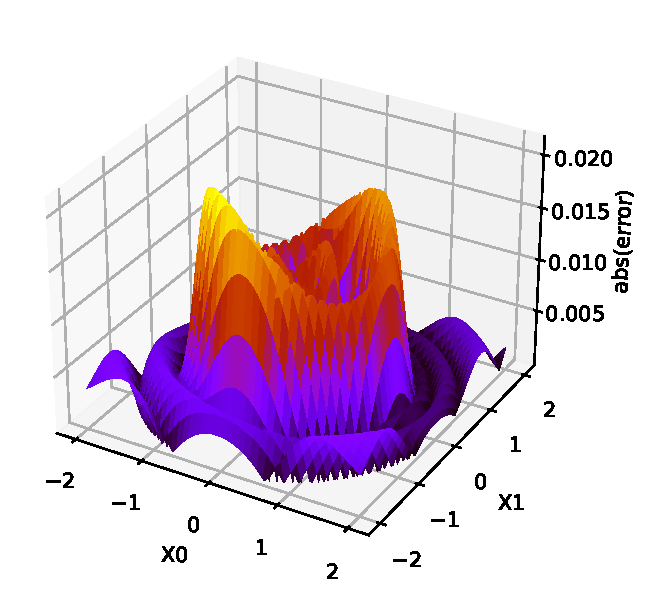
\includegraphics[width=1\textwidth]{../../code/experiments/experiment_3/pde0b_ex1_abs_error.pdf}
		\caption{Absolute error best\\ result using \gls{gak}. }
		\label{fig:pde0b_ex1_abs_error}
	\end{subfigure}% 
	%
	\begin{subfigure}[b]{0.4\linewidth}
		\centering
		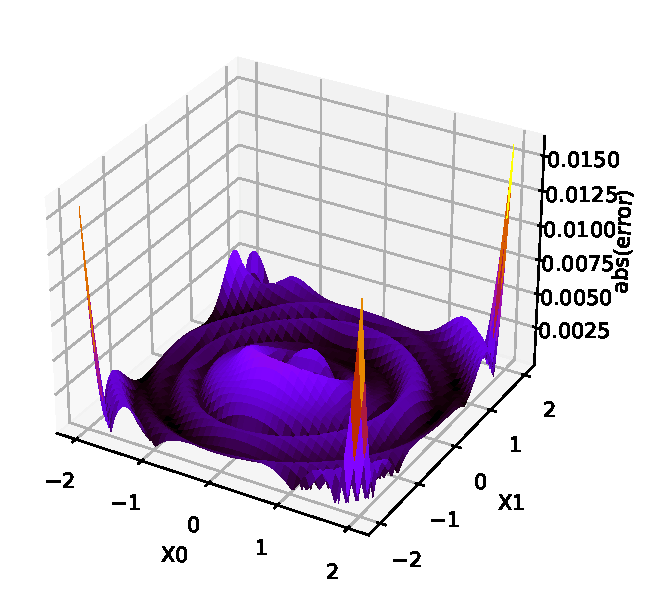
\includegraphics[width=1\textwidth]{../../code/experiments/experiment_3/pde0b_ex3_abs_error.pdf}
		\caption{Absolute error best\\ result using \gls{gsk}. }
		\label{fig:pde0b_ex3_abs_error}
	\end{subfigure}%
	\unterschrift{Comparisons of best solution absolute error by memetic parallel JADE using \gls{gak} and \gls{gsk} after $10^6$ \gls{nfe}.}{}{}%
	\label{fig:compare_abs_error_non_adaptive}
\end{figure}

\subsection{PDE 5}

The hypothesis of the \gls{gsk} is that it significantly increases the approximation quality of \gls{pde} 5. Further, it should overcome the phenomenon where the L2 norm increases with more \gls{nfe}. 

As table \ref{tab:compare_mpj_mpjgsk_10^6} shows, the results are indeed significantly better. Again, this can be confirmed from a visual perspective by looking at the 3D plot of the approximation. Figure \ref{fig:pde5_ex3_compare_best_worst} depicts the best and the worst approximation of the 20 replications. Although the results are clearly better and the global structure is described more accurately, the \gls{ci} solver can not compete with the \gls{fem} solver. 


\begin{figure}[H]
	\centering
	\begin{subfigure}[b]{0.3333\linewidth}
		\centering
		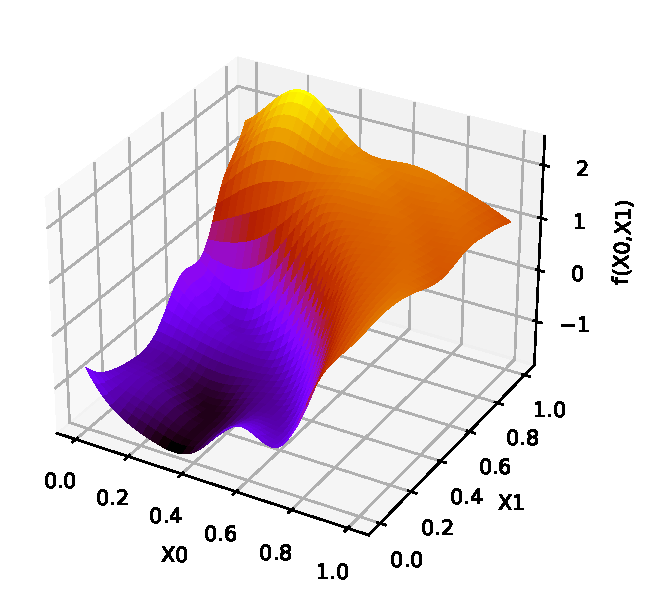
\includegraphics[width=1\textwidth]{../../code/experiments/experiment_3/pde5_best_solution_non-adaptive.pdf}
		\caption{best run  \gls{gsk} \\L2 norm: 0.252574}
		\label{fig:pde5_ex3_worst_solution_non-adaptive}
	\end{subfigure}% 
	%
	\begin{subfigure}[b]{0.3333\linewidth}
		\centering
		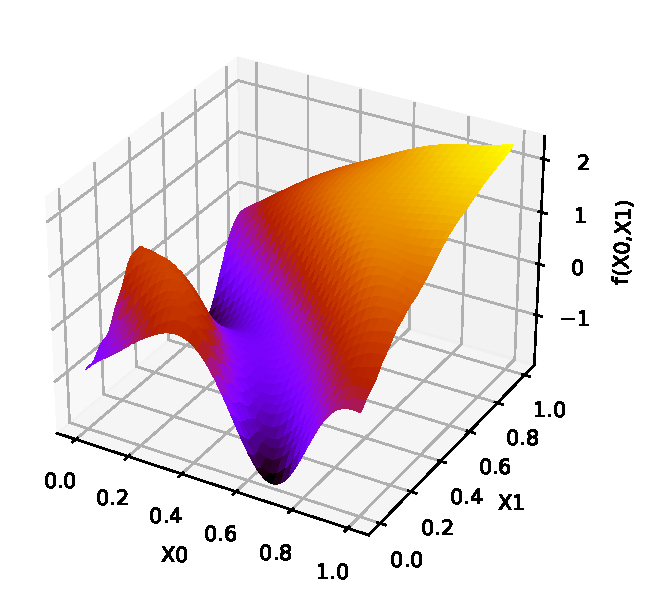
\includegraphics[width=1\textwidth]{../../code/experiments/experiment_3/pde5_worst_solution_non-adaptive.pdf}
		\caption{worst run \gls{gsk} \\L2 norm: 0.883869}
		\label{fig:pde5_ex3_best_solution_adaptive}
	\end{subfigure}%
	%
	\begin{subfigure}[b]{0.3333\linewidth}
		\centering
		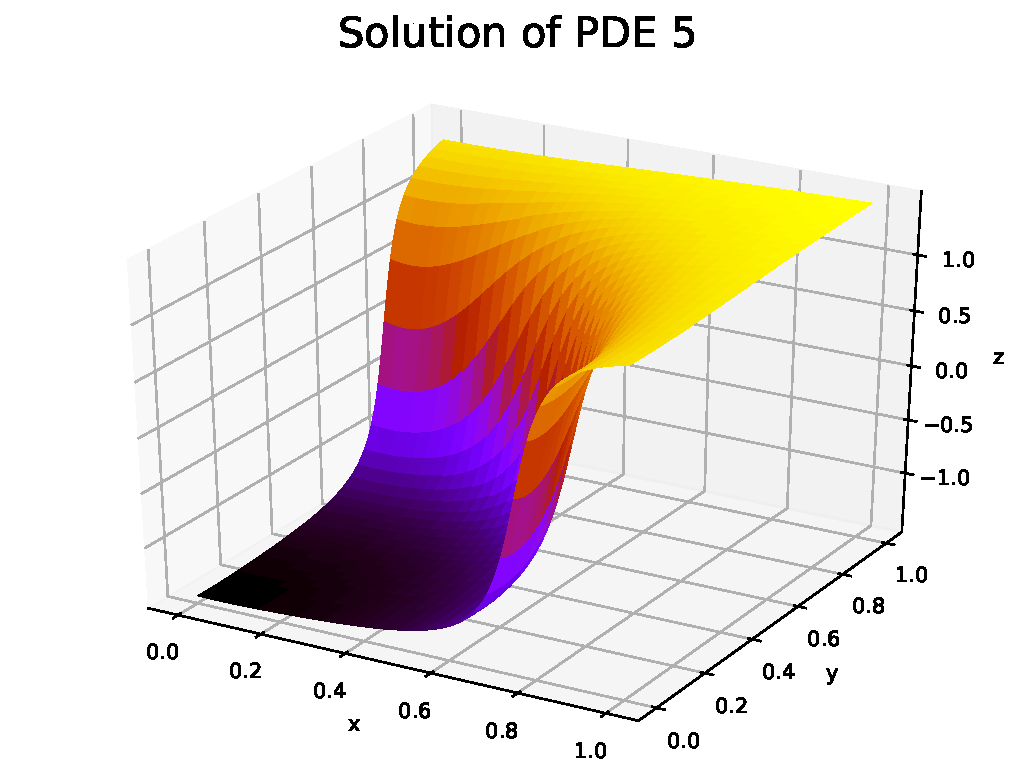
\includegraphics[width=1\textwidth]{../../code/testbed/pde5/sol_pde_5.pdf}
		\caption{analytical solution \\to \gls{pde} 5.}
		\label{fig:pde5_analytical_solution_3}
	\end{subfigure}%
	\unterschrift{Comparison of the best and the worst result generated by memetic pJADE with \gls{gsk} after $10^6$ \gls{nfe}. }{}{}%
	\label{fig:pde5_ex3_compare_best_worst}
\end{figure}

The following histograms in figure \ref{fig:pde5_L2norm_histogram_gsk} compare the experimental distribution of the L2 norm with the \gls{gak} and the \gls{gsk}. As inferred from the Wilcoxon test, the distributions are significantly different. Further, the mean and the median of the ``\gls{gsk}-data'' is smaller than the same statistical indicators of the ``\gls{gak}-data''. 

The histogram of the fitness values is shown in figure \ref{fig:pde5_fitness_histogram_gsk}. Contrary to the exception, the fitness values of the \gls{gak} are smaller than the fitness values of the \gls{gsk}. Because the fitness function changed with the usage of the \gls{gsk}, the numerical values can not be compared directly. 

\begin{figure}[H]
	\centering
	\begin{subfigure}[b]{0.5\linewidth}
		\centering
		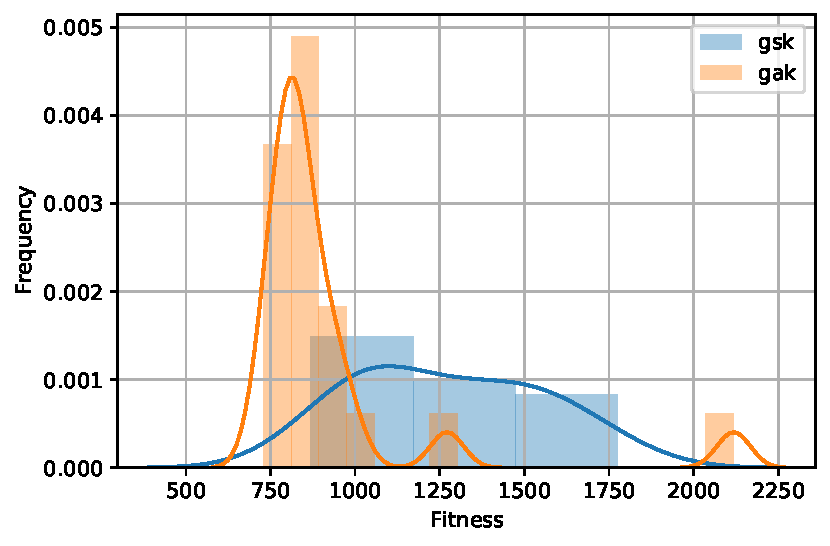
\includegraphics[width=1\textwidth]{../../code/experiments/experiment_3/pde5_non-adaptive_histogram_fit.pdf}
		\caption{Histogram of fitness value using \gls{gsk} and \gls{gak}.}
		\label{fig:pde5_fitness_histogram_gsk}
	\end{subfigure}%
	%
	\begin{subfigure}[b]{0.48\linewidth}
		\centering
		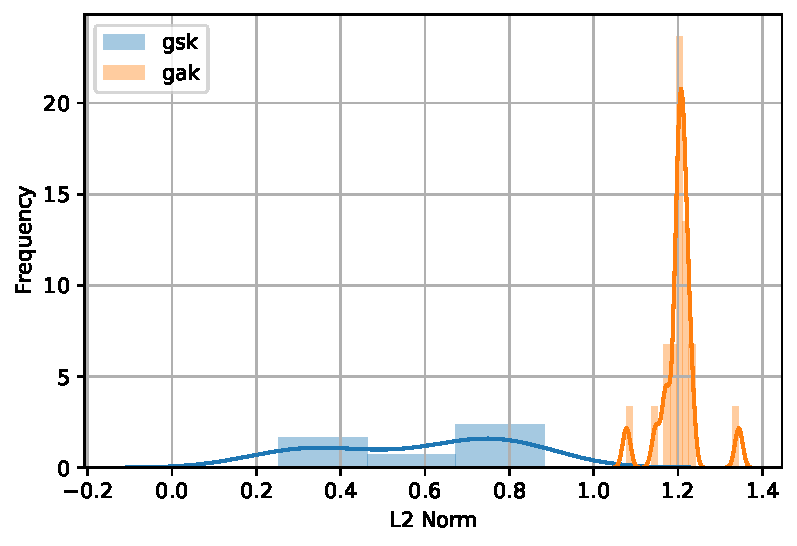
\includegraphics[width=1\textwidth]{../../code/experiments/experiment_3/pde5_non-adaptive_histogram_L2.pdf}
		\caption{Histogram of L2 norm using \gls{gsk} and \gls{gak}.}
		\label{fig:pde5_L2norm_histogram_gsk}
	\end{subfigure}% 
	\unterschrift{Histograms of \gls{gsk} and \gls{gak} L2 norm and fitness value on \gls{pde} 5 after $10^6$ \gls{nfe}. }{}{}%
	\label{fig:pde5_ex3_histogram}
\end{figure}

Similar to the plot in chapter \ref{chap:ex0_pde5}, figure \ref{fig:ex3_pde5_gsk_fit_vs_l2} connects the L2 norm of one individual with its fitness value at every generation. Although the effect of a raising L2 norm with increasing \gls{nfe} is mitigated, it can be seen that the best quality is not reached after $10^6$ \gls{nfe}. After generation 5000, the L2 norm settles in at around 0.4, while the fitness value continues to decrease. 

\begin{figure}[H]
	\centering
	\noindent\adjustbox{max width=0.7\linewidth}{
		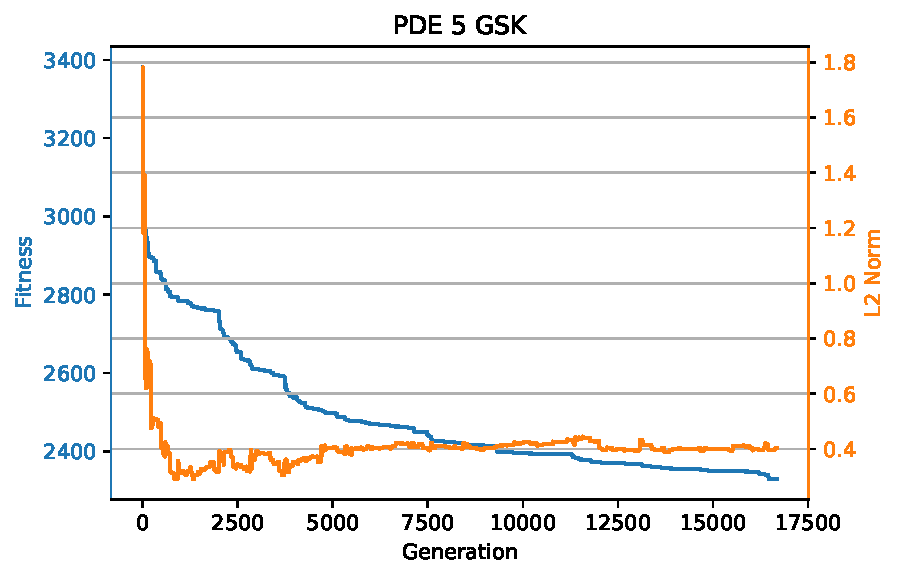
\includegraphics[width=\textwidth]{../../code/experiments/misc/pde5_gsk_fit_l2_history.pdf}
	}
	\unterschrift{Fitness value and L2 Norm of an exemplary individual at every generation on \mbox{\gls{pde} 5} using a \gls{gsk}. }{}{}
		\label{fig:ex3_pde5_gsk_fit_vs_l2}
\end{figure}
	
This again shows that a good fitness value does not necessarily indicate a good approximation quality. Although this property is only shown on \gls{pde} 5, it might also be true on other \gls{pde}s. This issue demonstrates that the fitness function suffers from a fundamental problem, but currently this is the best indicator for good solutions that only use the information posed in the original problem definition. It can be concluded that choosing an appropriate kernel is not trivial, especially in the common case where the analytical solution to the \gls{pde} is not known.  

\end{document}